%!TEX root = ./thesis.tex

% \chapter{Template}\label{chapter:kapitellabel} %%%%%%%%%%%%%%%%%%%%%%%%%%%%
% \section{Test}
% \subsection{Sub Test}
% Itaque earum rerum hic tenetur a sapiente delectus, ut aut reiciendis voluptatibus maiores alias consequatur aut perferendis doloribus asperiores repellat\cite{aho:dragonbook}. See Table ~\ref{table:speedup1} and ~\ref{table:speedup1} and \ref{figure:helloworld}.

% \begin{table}[!th]
%   \renewcommand{\arraystretch}{1.3}
%   \caption{Speed-Up Table I}\label{table:speedup1}
%   \vspace{4mm} % hack
%   \centering
%     \begin{tabular}{|l||r|r|r|}
%       \hline
%       program            & basline   & algorithm 1  & alogrithm 2\\
%       \hline
%       \hline
%       {\tt simple}       &  30 sec   &  20 sec      &  18 sec     \\
%       \hline
%       {\tt hello world}  &  43 sec   &  27 sec      &  28 sec     \\
%       \hline
%     \end{tabular}
% \end{table}

% \begin{table}[!th]
%   \renewcommand{\arraystretch}{1.3}
%   \caption{Speed-Up Table II}\label{table:speedup2}
%   \vspace{4mm} % hack
%   \centering
%     \begin{tabular}{|l||r|r|r|}
%       \hline
%       program            & basline   & algorithm 1  & alogrithm 2\\
%       \hline
%       \hline
%       {\tt simple}       &  30 sec   &  20 sec      &  18 sec     \\
%       \hline
%       {\tt hello world}  &  43 sec   &  27 sec      &  28 sec     \\
%       \hline
%     \end{tabular}
% \end{table}
% Lorem ipsum dolor sit amet, consectetur adipiscing elit, sed do eiusmod tempor incididunt ut labore et dolore magna aliqua. Ut enim ad minim veniam, quis nostrud exercitation ullamco laboris nisi ut aliquip ex ea commodo consequat. Duis aute irure dolor in reprehenderit in voluptate velit esse cillum dolore eu fugiat nulla pariatur. Excepteur sint occaecat cupidatat non proident, sunt in culpa qui officia deserunt mollit anim id est laborum

% \begin{figure}[!ht]
% \centering
% \sourcecode{main.cpp}
% \caption{Hello World Program}\label{figure:helloworld}
% \end{figure}
% Lorem ipsum dolor sit amet, consectetur adipiscing elit, sed do eiusmod tempor incididunt ut labore et dolore magna aliqua. Ut enim ad minim veniam, quis nostrud exercitation ullamco laboris nisi ut aliquip ex ea commodo consequat. Duis aute irure dolor in reprehenderit in voluptate velit esse cillum dolore eu fugiat nulla pariatur. Excepteur sint occaecat cupidatat non proident, sunt in culpa qui officia deserunt mollit anim id est laborum

% Lorem ipsum dolor sit amet, consectetur adipiscing elit, sed do eiusmod tempor incididunt ut labore et dolore magna aliqua. Ut enim ad minim veniam, quis nostrud exercitation ullamco laboris nisi ut aliquip ex ea commodo consequat. Duis aute irure dolor in reprehenderit in voluptate velit esse cillum dolore eu fugiat nulla pariatur. Excepteur sint occaecat cupidatat non proident, sunt in culpa qui officia deserunt mollit anim id est laborum~\cite{GorillaArm}

% \begin{figure}[!ht] % see https://en.wikibooks.org/wiki/LaTeX/Floats,_Figures_and_Captions for placement parameters
%   \centering
%   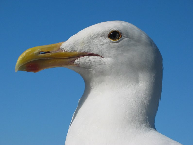
\includegraphics[width=0.5\textwidth]{images/gull.png}
%   \caption{A picture of a gull.}
% \end{figure}

% Lorem ipsum dolor sit amet, consectetur adipiscing elit, sed do eiusmod tempor incididunt ut labore et dolore magna aliqua. Ut enim ad minim veniam, quis nostrud exercitation ullamco laboris nisi ut aliquip ex ea commodo consequat. Duis aute irure dolor in reprehenderit in voluptate velit esse cillum dolore eu fugiat nulla pariatur. Excepteur sint occaecat cupidatat non proident, sunt in culpa qui officia deserunt mollit anim id est laborum

% Lorem ipsum dolor sit amet, consectetur adipiscing elit, sed do eiusmod tempor incididunt ut labore et dolore magna aliqua. Ut enim ad minim veniam, quis nostrud exercitation ullamco laboris nisi ut aliquip ex ea commodo consequat. Duis aute irure dolor in reprehenderit in voluptate velit esse cillum dolore eu fugiat nulla pariatur. Excepteur sint occaecat cupidatat non proident, sunt in culpa qui officia deserunt mollit anim id est laborum

% Lorem ipsum dolor sit amet, consectetur adipiscing elit, sed do eiusmod tempor incididunt ut labore et dolore magna aliqua. Ut enim ad minim veniam, quis nostrud exercitation ullamco laboris nisi ut aliquip ex ea commodo consequat.
% \begin{figure}[H]
%   \centering
%   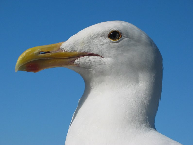
\includegraphics[width=0.5\textwidth]{images/gull.png}
%   \caption{A picture of a gull.}
% \end{figure}
% Duis aute irure dolor in reprehenderit in voluptate velit esse cillum dolore eu fugiat nulla pariatur. Excepteur sint occaecat cupidatat non proident, sunt in culpa qui officia deserunt mollit anim id est laborum

% Lorem ipsum dolor sit amet, consectetur adipiscing elit, sed do eiusmod tempor incididunt ut labore et dolore magna aliqua. Ut enim ad minim veniam, quis nostrud exercitation ullamco laboris nisi ut aliquip ex ea commodo consequat. Duis aute irure dolor in reprehenderit in voluptate velit esse cillum dolore eu fugiat nulla pariatur. Excepteur sint occaecat cupidatat non proident, sunt in culpa qui officia deserunt mollit anim id est laborum

\chapter{Einführung}\label{chapter:kapitellabel}

Zweibeiniges Gehen bietet als Fortbewegungsart durch virtuelle Realität viele Vorteile gegenüber alternativen Fortbewegungsarten.[

    %TODO:Quelle
    ]
beschreibt beispielsweise, ein höheres Präsensgefühl der Nutzer:innen.[
    %TODO: Quelle

]
zeigt dass weniger Motion sickness entsteht wenn sich die Nutzer:innen durch die virtuelle Welt bewegen indem sie gehen.
[
    %TODO: quelle

]
erklärt das beim Gehen mehr Sinne stimuliert werden als bei künstlichen Alternativen, wie zum Beispiel der Joystick Steuerung. Tiefensensibilität (Propriozeption) und Gleichgewichtssinn (vestibuläre Wahrnehmung) signalisieren, dass er gerade wirklich geht, während diese Information bei alternativen Fortbewegungsart allein vom visuellen Sinn übermittelt wird.
Leider bring das reale gehen (real walking nach[
    %TODO: quelle

]
) auch den großen Nachteil mit sich, dass es in der Regel auf einen einzelnen Raum (den Trackingspace) beschränkt ist. Zwar gibt es dazu auch ausnahmen, ( siehe z.B.[
    %TODO: quelle microsoft studie
]
), jedoch sind diese dann mit großem Aufwand verbunden und nicht für jede Endnutzer:in umzusetzen.

\section{Redirected Walking}
%sind impossible spaces überhaupt redirected walking?
Eine Art dieses Problem zu Umgehen ist das so genannte \textquote{Redirected Walking}. Dies ist eine Sammlung von Techniken mit denen die Nutzer:in subtilen Manipulationen der Fortbewegungsart durch den Trackingspace navigiert wird. Dabei wird die Illusion aufrecht erhalten sie würde sich unverändert, frei bewegen. So lässt sich die Nutzer:in von den äußeren Begrenzungen des Trackingspaces fern halten, und die virtuell begehbare Fläche vergrößern.
Im folgenden werde ich nun zwei dieser Techniken genauer vorstellen.

\subsection{Rotation Gains}
%TODO: quelle steinicke zusammenfassung der techniken
Rotation Gains werden Kopfrotationen hinzugefügt sodass sich die virtuelle Kamera leicht schneller oder langsamer dreht als der reale Kopf mit dem VR-Headset. Kopfrotationen lassen sich mit der Schreibweise Rreal :=
(pitchreal, yawreal, rollreal)
%TODO: latex formatting
darstellen, wobei pitch, yaw und roll
%TODO: latex formatting
die Eulerschen Winkel der Kopfrotation darstellen. Für alle 3 Winkel kann ein rotation gain angewandt werden. Der rotation gain wird dann als Quotient des virtuellen Winkels und des realen Winkels definiert also: gR := Rvirtual / Rreal
%TODO: latex formatting.
Dieses Anwenden funktioniert indem der rotation gain gR mit dem Winkel der realen Kopfrotation (alpha) multipliziert wird also: gR * alpha
%TODO: latex formatting.
Da für jeden Winkel der Kopfrotation ein rotation gain definiert werden kann werden Rotationgains folgendermaßen dargestellt: (gRpitch, gRyaw, gRroll)



\subsection{Impossible Spaces}

\chapter{Verwandte Arbeiten}\label{chapter:kapitellabel}

\chapter{Generierte Level}\label{chapter:kapitellabel}

\chapter{Fortbewegungsarten}\label{chapter:kapitellabel}

\chapter{Implementierung}\label{chapter:kapitellabel}

\chapter{Experiment}\label{chapter:kapitellabel}

\chapter{Teilnehmer}\label{chapter:kapitellabel}

\chapter{Materialien}\label{chapter:kapitellabel}

\chapter{Methoden}\label{chapter:kapitellabel}

\chapter{Ergebnisse}\label{chapter:kapitellabel}

\chapter{Diskussion}\label{chapter:kapitellabel}

\chapter{Konklusion}\label{chapter:kapitellabel}

\chapter{Acknowledgments}\label{chapter:kapitellabel}


% keep an blank line above
